\subsection{Syntax units}

\begin{figure}[b]
    \centering
    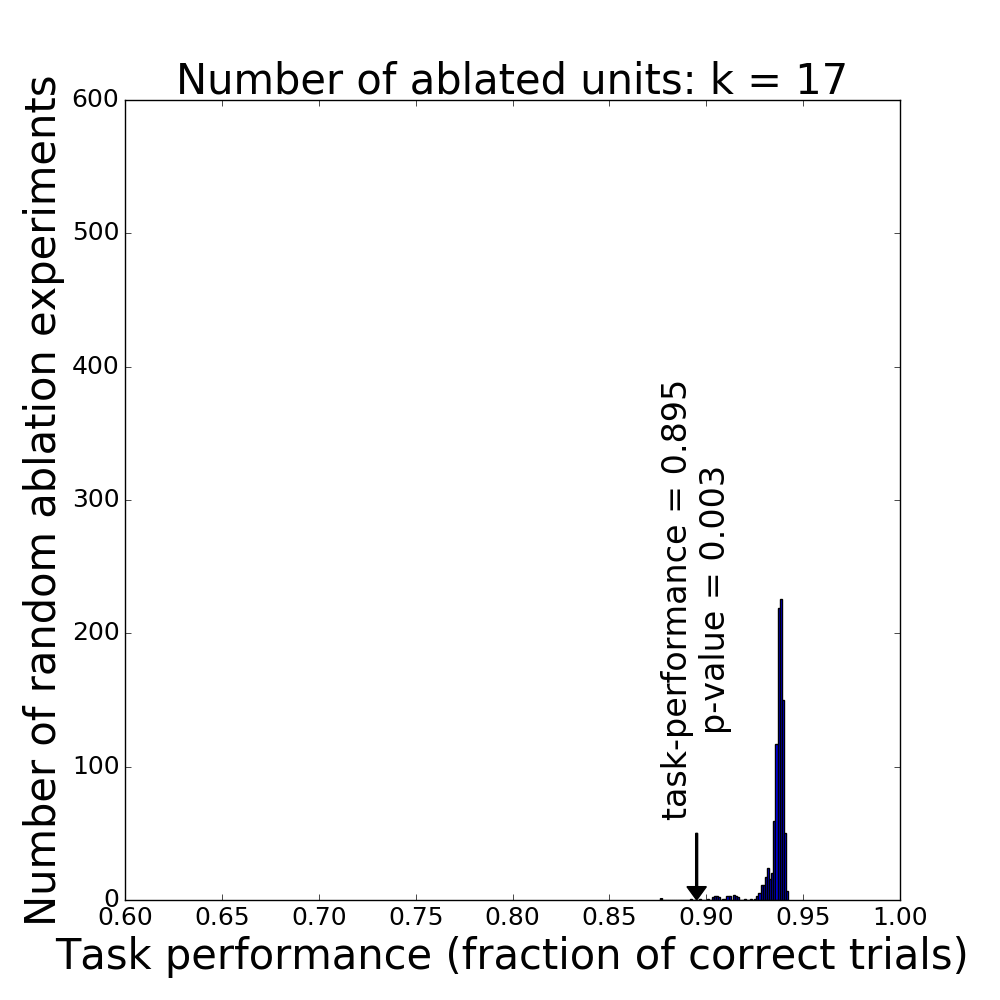
\includegraphics[height=5cm]{Figures/null_distribution_ablation_experiment_k_17.png}
    \caption{Network performance}
    \label{fig:ablation-syntax}
\end{figure}

\begin{figure}[ht]
    \begin{subfigure}{\linewidth}
            \centering
            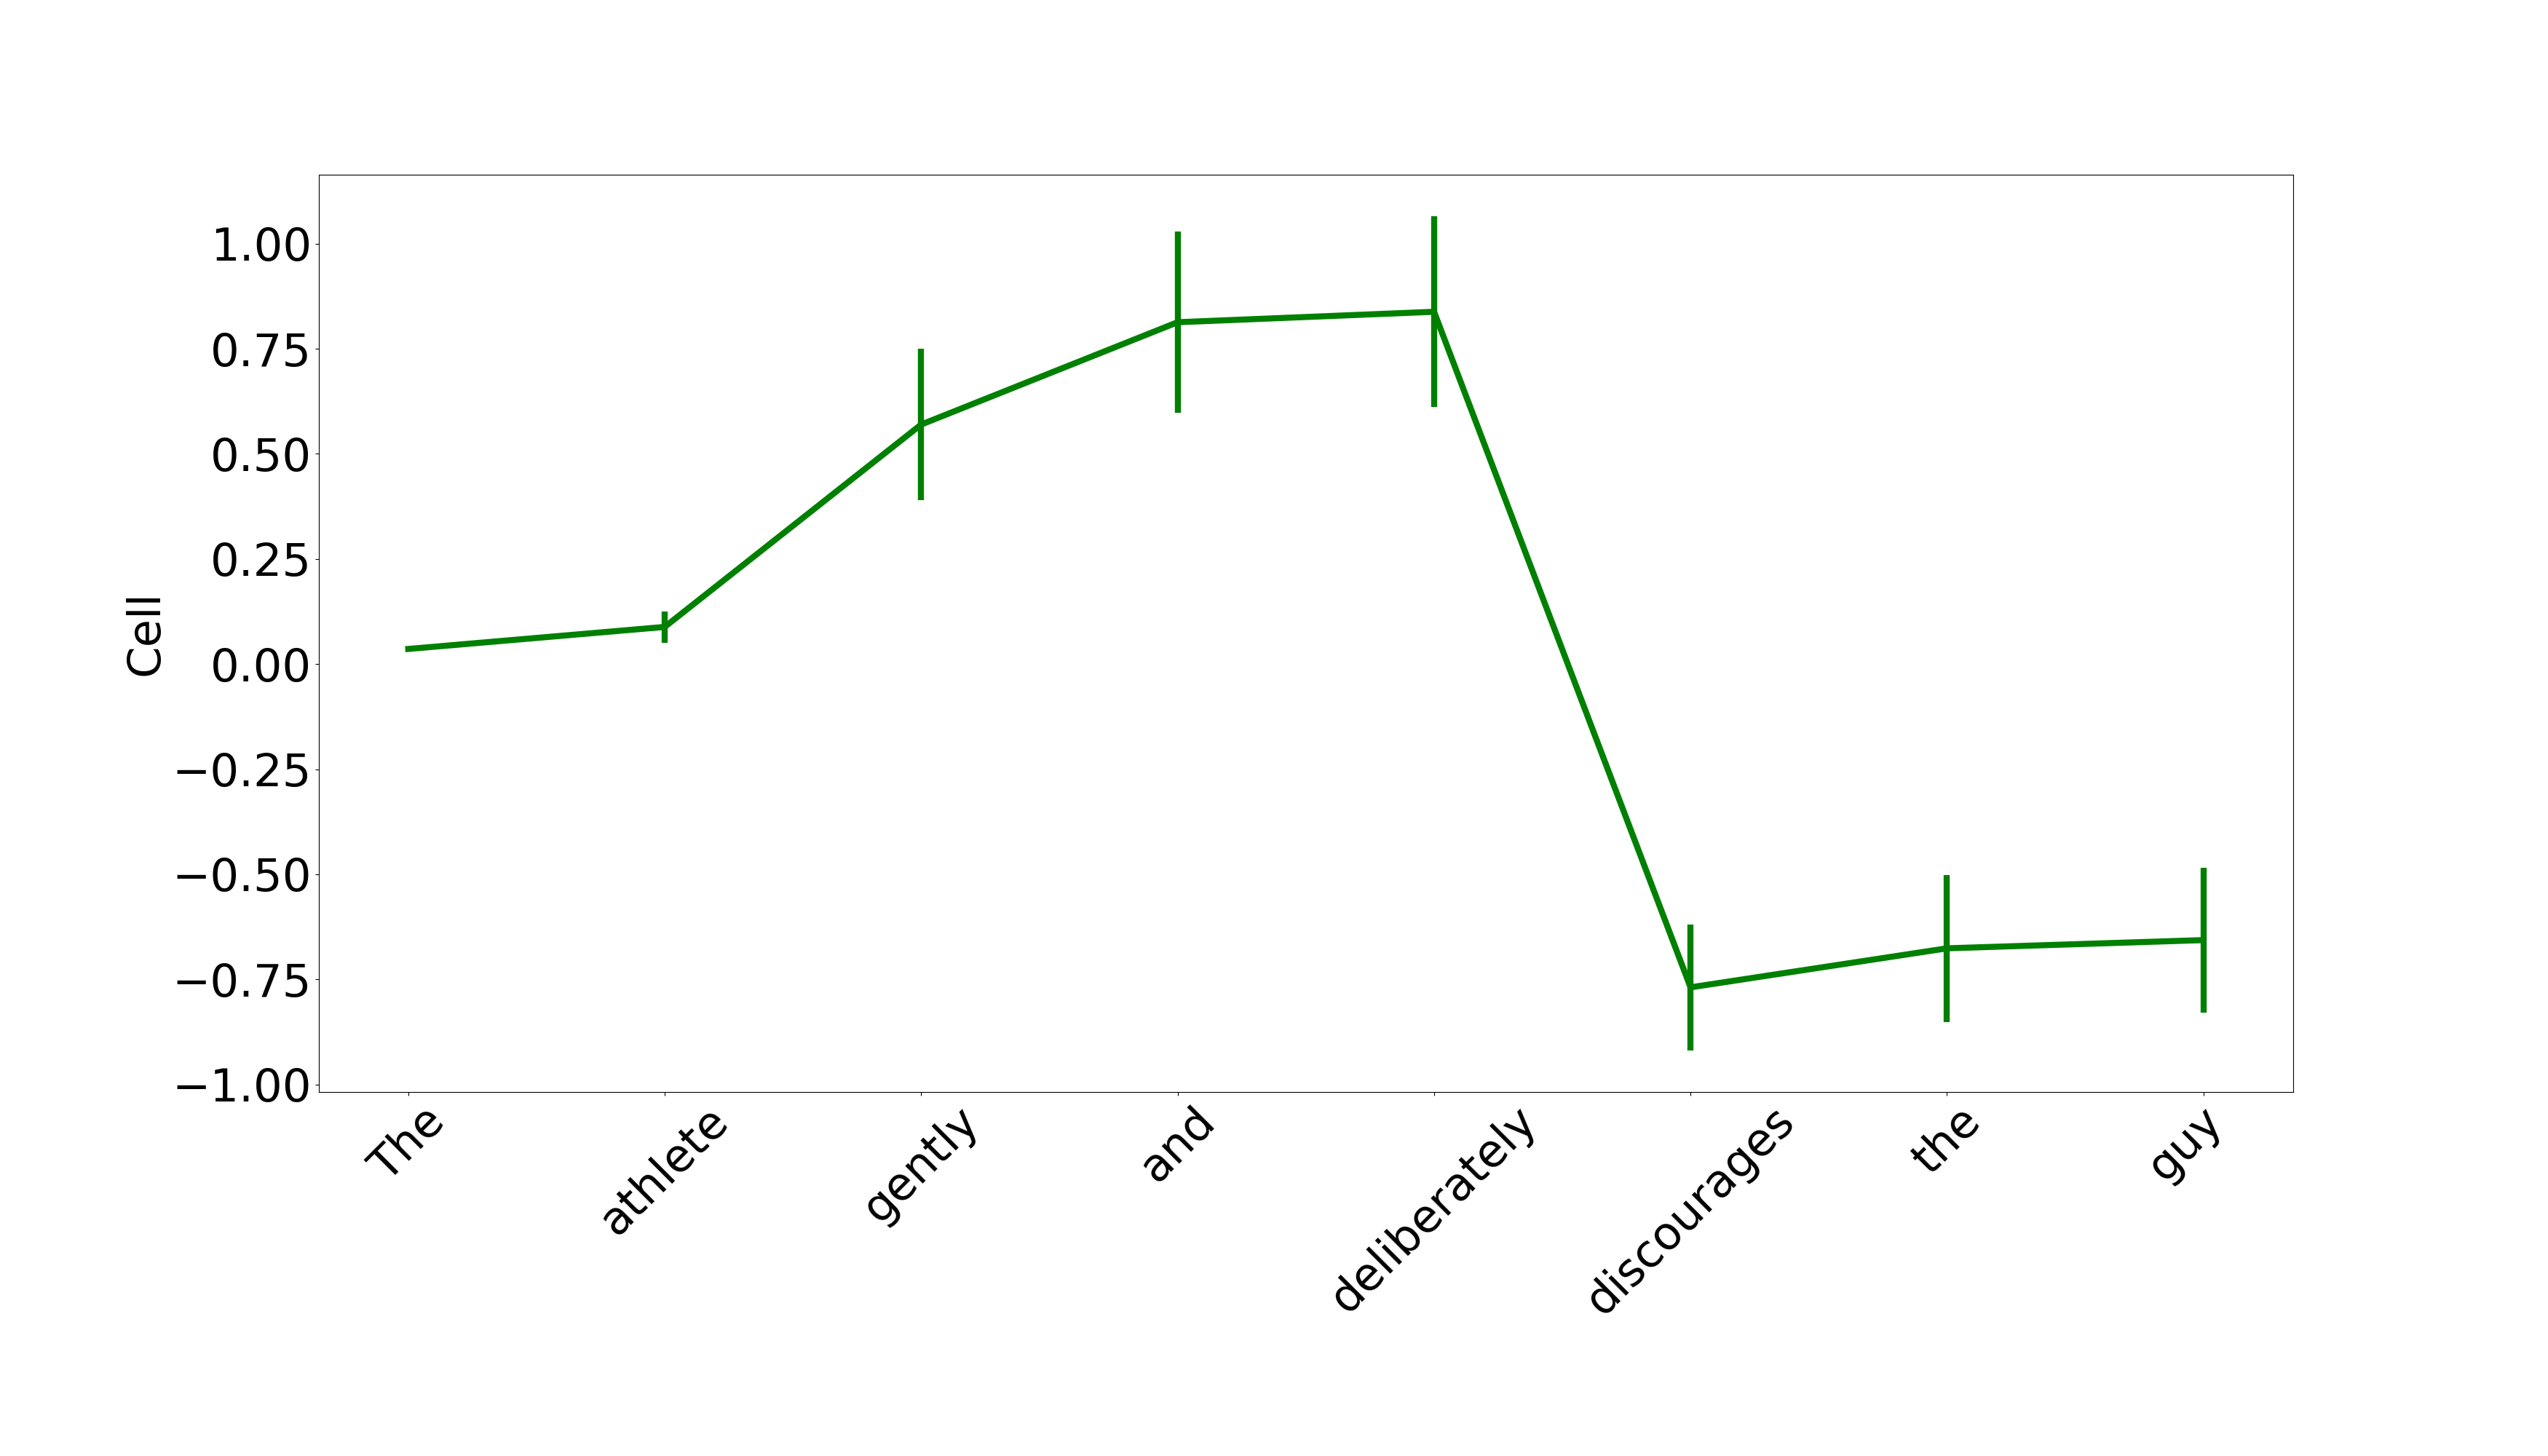
\includegraphics[width=\linewidth, height=2cm]{Figures/adv_conjunction_1149_cell}
            \caption{2Adv}
            \label{fig:syntax-unit-2Adv}
    \end{subfigure}
    \begin{subfigure}{\linewidth}
            \centering
            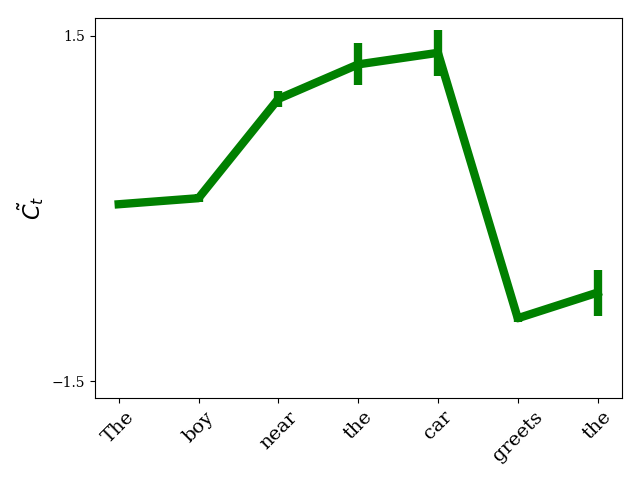
\includegraphics[width=\linewidth, height=2cm]{Figures/nounpp_1149_cell.png}
            \caption{nounPP}
            \label{fig:syntax-unit-nounpp}
    \end{subfigure}
    \begin{subfigure}{\linewidth}
            \centering
            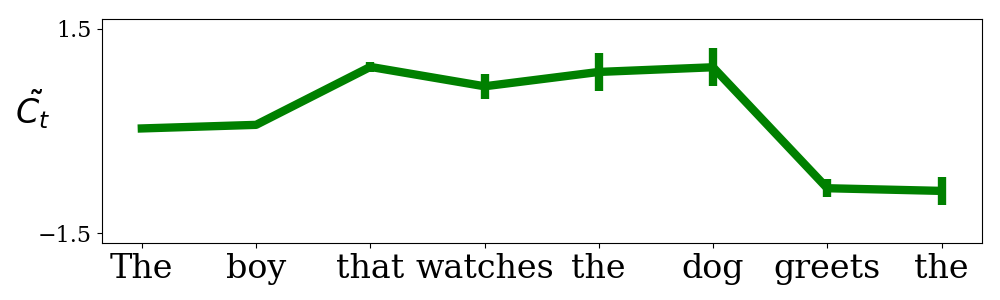
\includegraphics[width=\linewidth, height=2cm]{Figures/subjrel_that_1149_cell.png}
            \caption{subject relative}
            \label{fig:syntax-unit-subjrel}
    \end{subfigure}
    \begin{subfigure}{\linewidth}
            \centering
            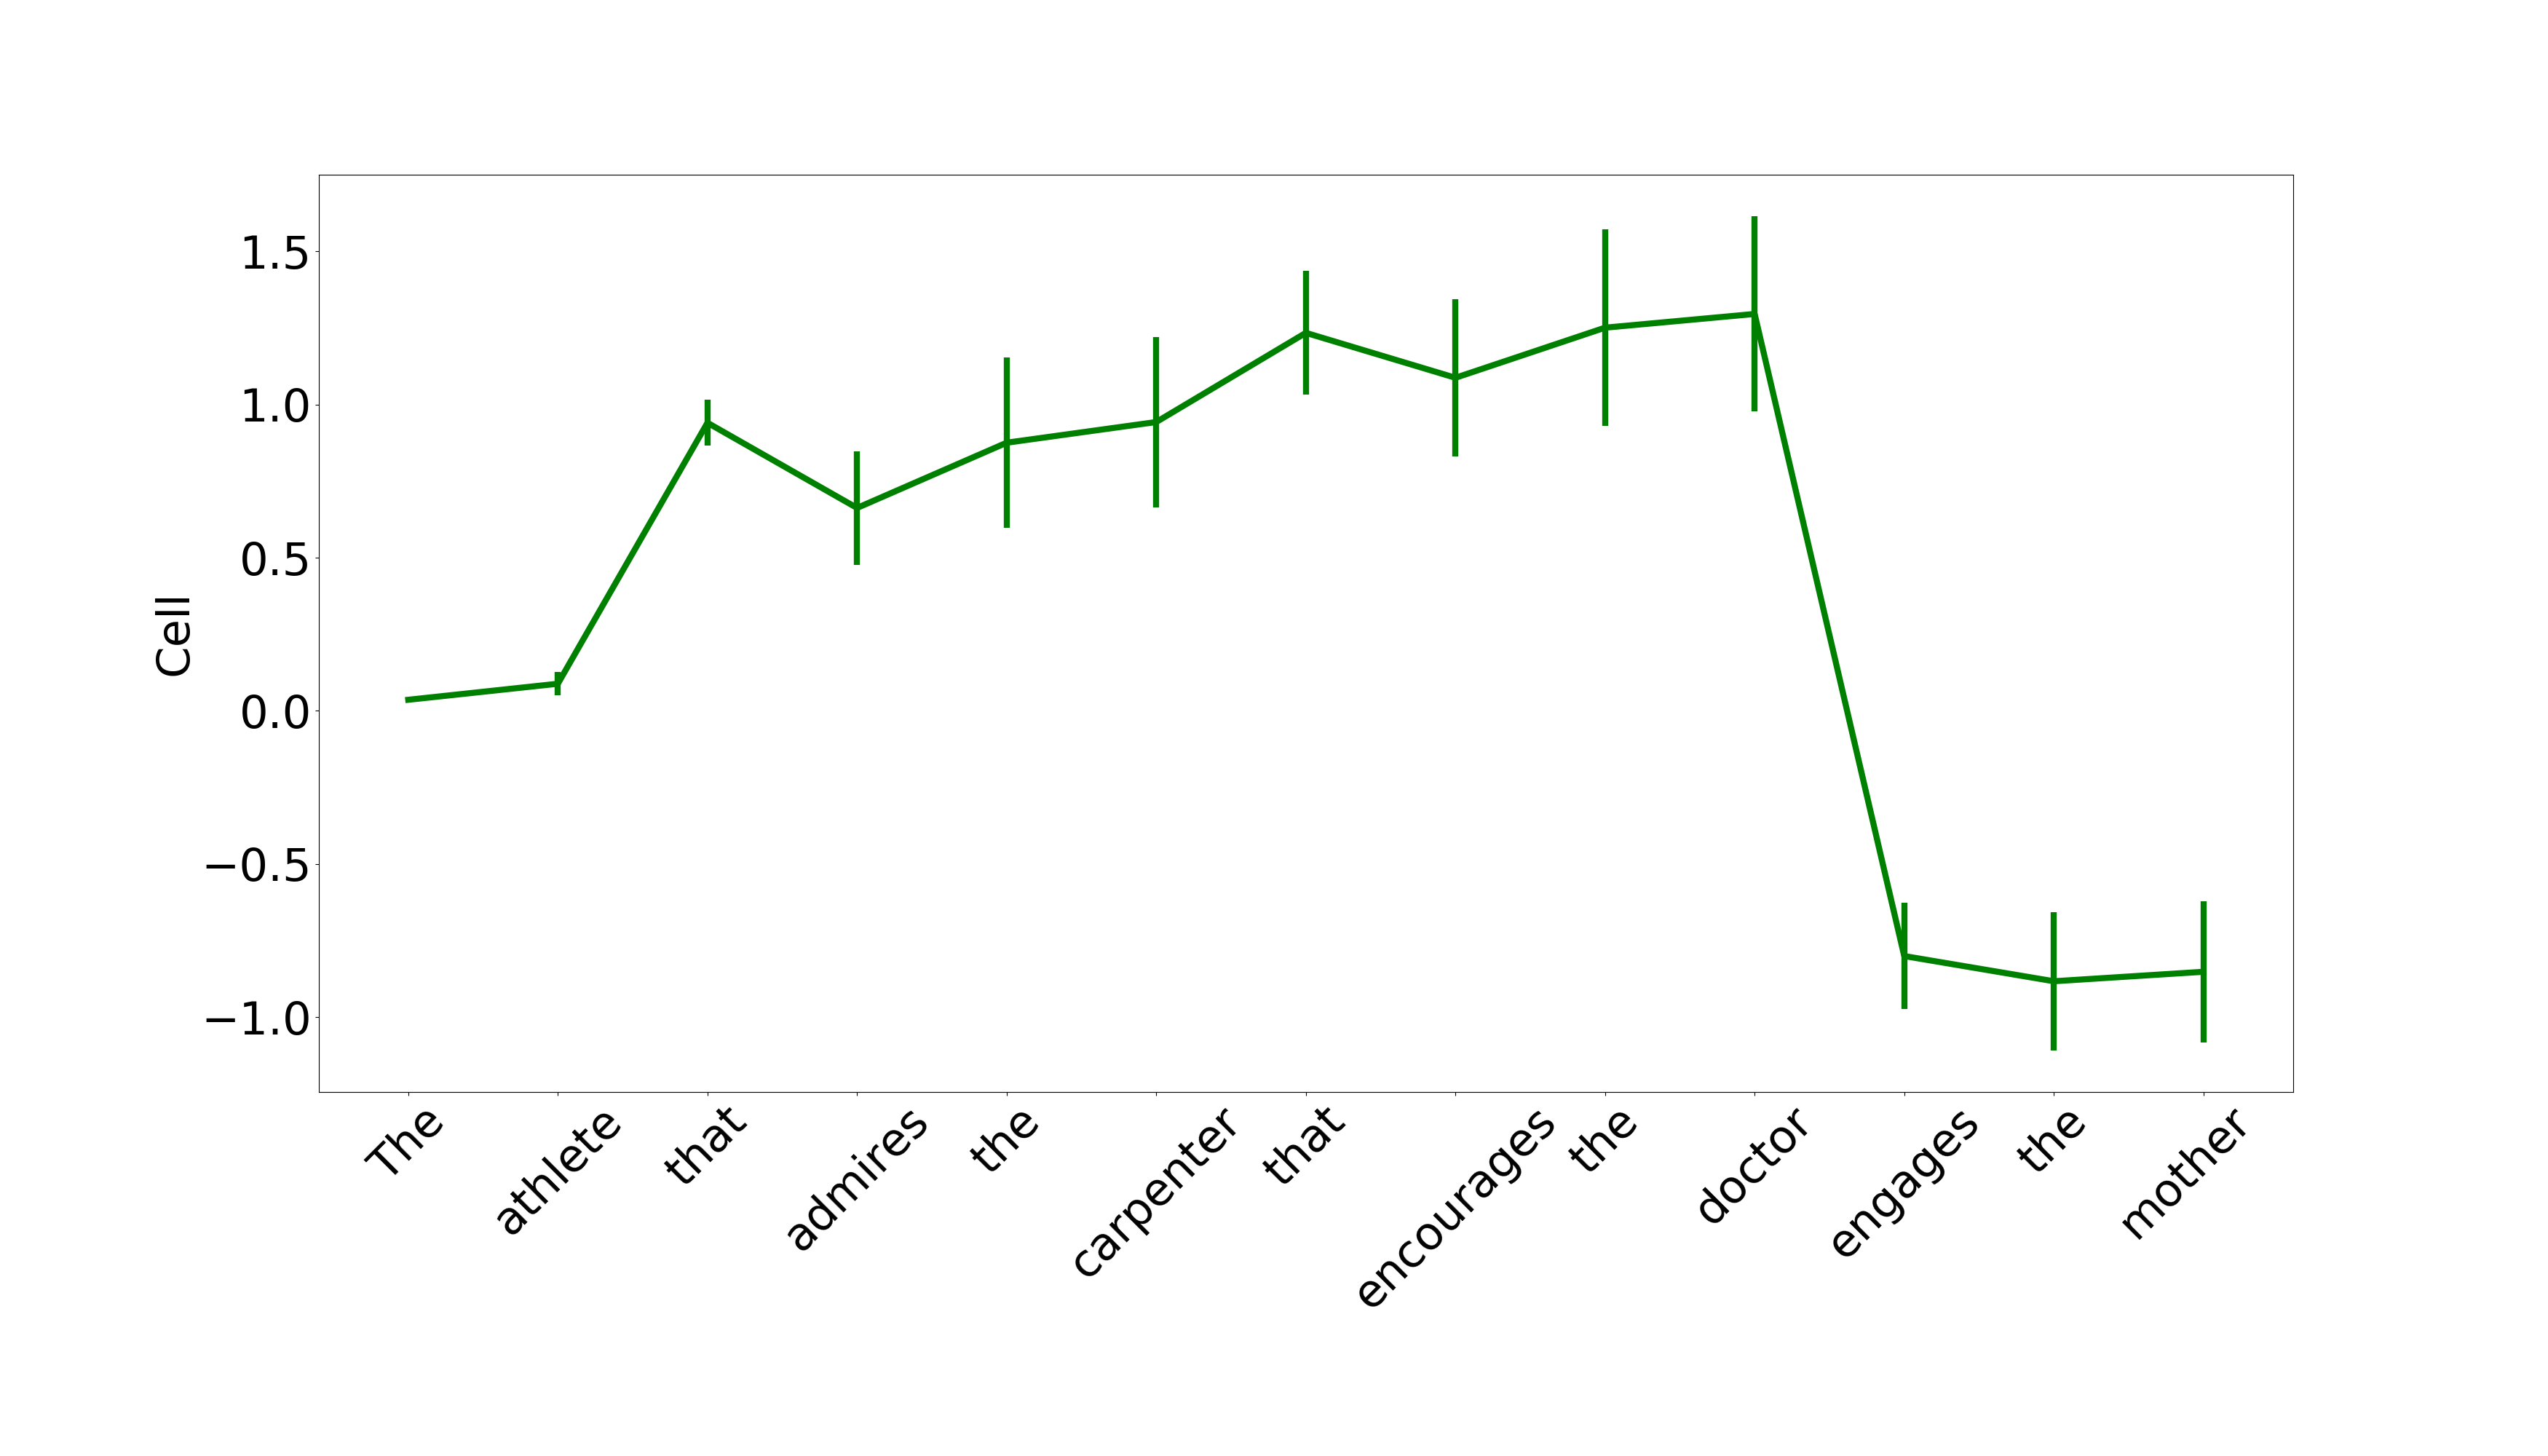
\includegraphics[width=\linewidth, height=2cm]{Figures/double_subjrel_that_1149_cell.png}
            \caption{Two embeddings with subject relatives}
            \label{fig:syntax-unit-double-subjrel}
    \end{subfigure}
\caption{Cell activity of the syntax unit 1150 during the processing of various syntactic structures.}
\end{figure}


The previous section described how the input and forget gate of the singular and plural units control the storage of subject number in the cell. It remains unclear, however, how are the dynamics of these gates controlled by the network. We hypothesized that other units in the network may encode information about the syntactic structure of the sentence, and in particular, encode information regarding the subject-verb dependency. To explore this, we tested whether syntactic information can be decoded from other units in the network, by using the depth of the syntactic tree as a proxy for syntactic structure \yair{cite Nelson et. al 2017} and testing whether this information can be decoded from the pattern of activity of the network (section \ref{ssec:regress_model}). 

We found that syntactic tree-depth can be efficiently decoded from network activity \yair{mean R-squared + std}, and that a small subset of units resulted with relatively high weights \yair{number of units; outlier detection mean + 3std}, to which we will refer as syntax units. The syntax units were found to be crucial for accomplishing the NA-task, since ablating them resulted in significant performance reduction compared to 1000 random ablations of subsets of units of the same size ($p-value=0.024$), as seen in figure \ref{fig:ablation-syntax}. 

We next looked into the dynamics of these units by visualizing their gate and cell dynamics during sentence processing. We found that cell activity of one of the syntax units, unit 1150, which also had the highest weight in the regression study, was remarkably structured. Cell activity of this unit was found to increase across the entire subject-verb dependency and to abruptly drop right after. Figures \ref{fig:syntax-unit-2Adv} and \ref{fig:syntax-unit-nounpp} show cell activity of this unit during the processing of stimuli from the 2Adv and nounPP tasks. We further tested cell dynamics of this unit in cases where another verb appears before the main verb of the dependency as in subject-relatives (figure \ref{fig:syntax-unit-subjrel}), and in exceptionally LR dependencies with two interfering nouns and verbs before the main verb of the dependency (figure \ref{fig:syntax-unit-double-subjrel}). Taken together, these results suggest that the syntax unit 1150 consistently encodes the subject-verb dependency across various syntactic structures \footnote{Other syntax units didn't show an easily interpretable dynamics, nor interaction with the LR-units as shown below, but..}.